\documentclass[margin,center]{res}
\usepackage{hyperref}
\usepackage{url}
\usepackage{breqn}
\oddsidemargin -.5in
\evensidemargin -.5in
\textwidth=6.0in
\itemsep=0in
\parsep=0in
\topmargin=0in
\topskip=0in

\newenvironment{list1}{
  \begin{list}{\ding{113}}{%
      \setlength{\itemsep}{0in}
      \setlength{\parsep}{0in} \setlength{\parskip}{0in}
      \setlength{\topsep}{0in} \setlength{\partopsep}{0in}
      \setlength{\leftmargin}{0.17in}}}{\end{list}}
\newenvironment{list2}{
  \begin{list}{$\bullet$}{%
      \setlength{\itemsep}{0in}
      \setlength{\parsep}{0in} \setlength{\parskip}{0in}
      \setlength{\topsep}{0in} \setlength{\partopsep}{0in}
      \setlength{\leftmargin}{0.2in}}}{\end{list}}


    
\begin{document}
\name{\huge 
  Božidar Mitrović  }

\begin{figure}
\hfill\smash{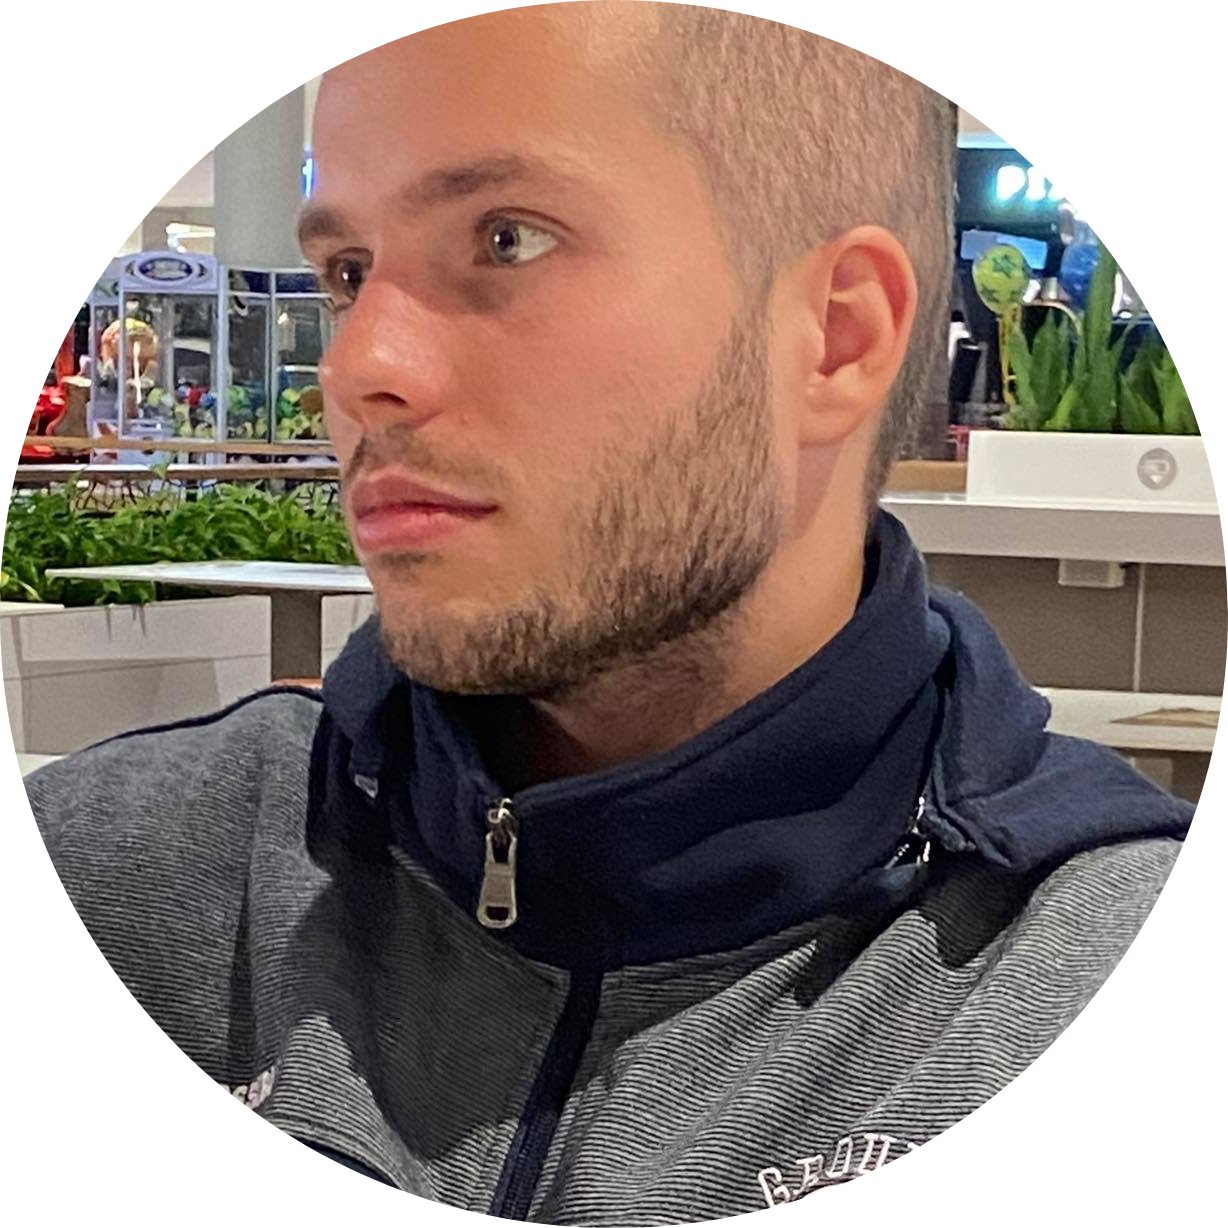
\includegraphics[height=2.5cm]{ja_round.png}}\vspace*{-1cm}
\end{figure}

\begin{resume}
\section{PERSONAL INFORMATION}
{ Email:    }   boza.mitrovic@gmail.com  \\ 
\href{https://github.com/AizenAngel}{Github}, \href{https://www.linkedin.com/in/bo%C5%BEidar-mitrovi%C4%87-1a379991/}{LinkedIn}


\section{EDUCATION}
{\bf Mathematical Grammar School} \hfill 2011 -- 2013\\
{\bf Mathematical Grammar School} \hfill 2013 -- 2017\\
{\bf University in Belgrade, Faculty of Mathematics}  \hfill 2017 -- 2021


\section{PROJECTS\\}
\begin{list2}
  \item{\bf Media Player} \hfill  Sep 2019\\
    Music player application for Android OS, implemented in Android Studio.
  \item{\bf Chat Application} \hfill Sep 2019\\
    Chat application for Android OS, implemented in Android Studio.
  \item{\bf AIBG 2.0} \hfill Aug 2019 -- Dec 2019 \\ 
    Organizer of Artificial Intelligence Battle Ground hackaton (AIBG).
  \item{\bf Statistical analysis of Titanic Dataset} \hfill April 2020\\
    Written in R Studio.  
  \item{\bf Face Recognition Software} \hfill June 2020\\
    Jupyter Notebook application that recognizes faces. Written in Tensorflow.
  \item{\bf Image Search Engine} \hfill Dec 2020 \\
    Image Search Engine Implementation in Python.
  \item{\bf FileBox}  \hfill Oct 2020 - Jan 2021\\
    Client-Server application that simulates cloud service. Written in C++.
  \item{\bf Analysis of \emph{The Office}} \hfill June 2021 \\
    Analysis of characters on the popular sitcom \emph{The Office}. Writen in Python.
  \item{\bf Buy\&Drive} \hfill March 2021 -- June 2021 \\
    Client-Server application for selling cars. Gained experience with: Angular11, PostgreSQL, TailwindCSS

\end{list2}

\section{COURSES}
\begin{list2}
  \item {\bf PSIML6} \hfill August 2020\\
    Petnica Summer Institute of Machine Learning (PSIML), where I
    advanced my knowledge and understanding of Machine Learning
    through intense all-day courses.

  \item {\bf RTRK Summer School of C++} \hfill August 2020\\
    Summer school, that gave me the opportunity to learn about the
    most significant changes in C++ language through theoretical and
    practical problems.

\end{list2}


\section{EXPERIENCE} 
\begin{list2}
  \item{\bf Teaching assistant at Educational Centre "Korak Napred"}  \hfill Aug 2018 --\\
    Teaching elementary and high school students math and programming and preparing them for competitions.
  \item{\bf Teaching assistant at "SystemPro"}  \hfill Sep 2019 --\\
    Teaching elementary and high school students programming technologies 
  \item{\bf YouTestMe Internship}  \hfill Okt 2019 -- Jan 2020\\
    Gained experience with JSF and PrimeFaces 7.0
\end{list2}

\section{COMPETITIONS}
\begin{list2}
\item{\bf SUMA Hackaton} \hfill April 2021\\
  Placed fourth on DataScience Hackaton organized by Student Union SUMA.
\end{list2}

\section{ABOUT ME}  
Graduated from the University in Belgrade, Faculty of Mathematics with a major in Informatics.
Have experience in coming out of my comfort zone, working under pressure, and giving 100\%.  
My hobbies are: perfumes, books, working-out, movies and comicbooks. 



\end{resume}
\end{document}